\newpage
\section{Theoretical Analysis}
\label{sec: analysis}
In this section, the circuit shown in Figure~\ref{fig:Circuit} is analysed
theoretically. \\
At first, we are going to explain the theoretical models we used to compute the outputs of the envelope detector and the voltage regulator.
After that, we will present plots of these outputs and the deviation of the output DC voltage from 12 Volts. 
Finally, we are able to compute the outuput DC level and the voltage ripple.

\subsection{Envelope detector}
\label{envelope}

\noindent The transformer of this circuit has a ratio of n:1 between the primary and secondary circuits, where n is greater than 1, meaning that:
 \begin{equation}
Amplitude_{secondary} = \frac{V_{PRIMARY}}{n}
  \label{eq:asecondary}
\end{equation}
\noindent For the envelope detector, the input voltage is the one in the secondary circuit:
 \begin{equation}
v_{SECONDARY} = \frac{V_{PRIMARY}}{n} cos(wt)
  \label{eq:vsecondary}
\end{equation}
\noindent For this circuit, we have choosen a full-wave bridge rectifier circuit, that is composed by four diodes, a resistance and a capacitor.
The output voltage in the envelope detector,$vo_{ENVELOPE}$, is the absolute value of the input voltage, in this case, $v_{SECONDARY}$, assuming the ideal model for diodes.
When the diode is on, $v_{SECONDARY}$ > $vo_{ENVELOPE}$ and when the diode is off $v_{SECONDARY}$ < $vo_{ENVELOPE}$.
From t = 0 until t = $t_{off}$, the diode is on and at $t_{off}$ the diode goes off, therefore, in this period of time:
\begin{equation}
vo_{ENVELOPE} = |v_{SECONDARY}|
  \label{eq:t < toff}
\end{equation}

\noindent To compute $t_{off}$, we used the following equation, where w = 2$\pi$f:
\begin{equation}
t_{off} = \frac{1}{w}atan(\frac{1}{wR_{enve}C})
  \label{eq:toff}
\end{equation}

\noindent From t = $t_{off}$ until the diode is on again:
\begin{equation}
vo_{ENVELOPE} = A_{secondary}|cos(wt)|e^{-\frac{t - t_{off}}{R_{enve}C}}
  \label{eq:t > toff}
\end{equation}

\noindent When the diode turns on again:
\begin{equation}
vo_{ENVELOPE} = |v_{SECONDARY}|
  \label{eq:t > ton}
\end{equation}

\noindent Also, at this moment, since full-wave rectifier circuit makes the output voltage the absolute value of the input voltage, 
the period of this circuit becomes half of the original period, reducing the time constant and our cost, therefore:
\begin{equation}
t_{off}new = t_{off} + \frac{1}{2f}
  \label{eq:new toff}
\end{equation}

\newpage
\subsection{Voltage Regulator}
\label{reg}
\noindent The voltage regulator is composed by a resistance and a limiter circuit. A limiter circuit is a serie of diodes, that, in this case, 
is a positive voltage limiter. Our goal is that the DC voltage, in the serie of diodes, is 12V. 
\noindent For the voltage regulator circuit, we have to separate the DC analysis and the incremental analysis.
\noindent At first, for the DC analysis, when $VO_{ENVELOPE}$ $\geq$ 12:
\begin{equation}
VO_{REGULATOR} = 12;
  \label{eq:dc1}
\end{equation}

\noindent On the other side, when $VO_{ENVELOPE}$ < 12:
\begin{equation}
VO_{REGULATOR} = VO_{ENVELOPE};
  \label{eq:dc2}
\end{equation}

\noindent Moving on to the incremental analysis, if $vo_{ENVELOPE}$ $\geq$ 12:
\begin{equation}
vo_{regulator} = \frac {n_{diodes}r_d}{n_{diodes}r_d + R_{reg}}(vo_{ENVELOPE} - average(vo_{ENVELOPE}))
  \label{eq:ac1}
\end{equation}
\noindent where $n_{diodes}$ is the number of diodes of the voltage regulator and $r_d$ is given by the following expression:
\begin{equation}
r_d = \frac{\eta V_T}{I_se^{\frac{v_{on}}{\eta V_T}}}
  \label{eq:rd}
\end{equation}
\noindent where $V_T$ is the thermal voltage (0,025 V), $\eta$ is the material constant (1), $I_s$ is the reverse saturation current (1*$10^{-14}$) 
and $v_{on}$ is given by the following equation:
\begin{equation}
v_{on} = \frac{12}{n_{diodes}}
  \label{eq:von}
\end{equation}
\noindent On the other side, if $vo_{ENVELOPE}$ < 12:
\begin{equation}
vo_{regulator} = vo_{ENVELOPE} - average(vo_{ENVELOPE})
  \label{eq:ac2}
\end{equation}

\newpage
\subsection{Results and plots obtained}
To calculate n from the transformer ratio n:1, we made an approximation using the diode equation to compute the current flowing in the diodes 
and in the resistance of the voltage regulator:
\begin{equation}
i = I_s(e^{\frac{12}{\eta V_T n_{diodes}}} - 1);
  \label{eq:id}
\end{equation}

\noindent Then, we calculated the voltage regulator input voltage and calculated n, using that. After, with this approximation, 
we adjust n in Ngspice, in order to obtain a lower ripple.

\noindent Therefore, the following table shows the values we choose for the circuit parameters.
\begin{table}[!h]
\centering
\begin{small}
\caption{Values of the circuit parameters} \label{Table1}
\begin{tabular}{|c|c|}
\hline
$n_{diodes}$  & \partialinput{1}{1}{tabelaValues.tex}\\
$n$   & \partialinput{2}{2}{tabelaValues.tex} \\
$C$   & \partialinput{3}{3}{tabelaValues.tex} \\
$R_{env}$    & \partialinput{4}{4}{tabelaValues.tex} \\
$R_{reg}$    & \partialinput{5}{5}{tabelaValues.tex} \\
\hline
\end{tabular}
\end{small}
\end{table}

\noindent With this parameters, we have obtained the following values:
\begin{table}[!h]
\centering
\begin{small}
\caption{Results obtained} \label{Table2}
\begin{tabular}{|c|c|}
\hline
$average(v_O)$  & \partialinput{1}{1}{tabela1.tex}\\
$Ripple$   & \partialinput{2}{2}{tabela1.tex} \\
$average(|v_O - 12)|)$   & \partialinput{3}{3}{tabela1.tex} \\
$cost$    & \partialinput{4}{4}{tabela1.tex} \\
$Merit$    & \partialinput{5}{5}{tabela1.tex} \\
\hline
\end{tabular}
\end{small}
\end{table}

\noindent At last, the following plots show our results graphically.

\begin{figure}[h!] \centering
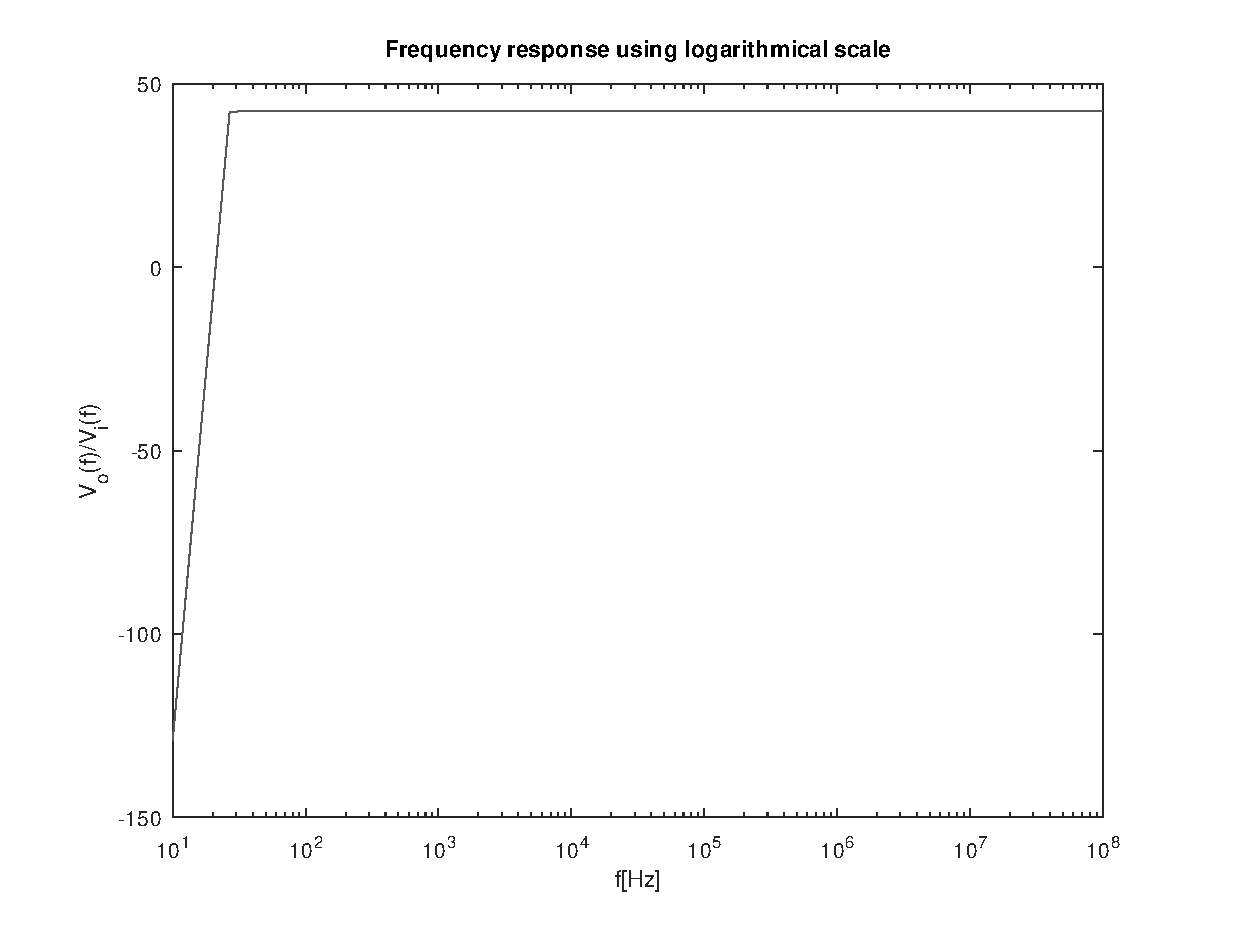
\includegraphics[width=0.7\linewidth]{plot1.eps}
\caption{$vo_{ENVELOPE}$ in Volts.}
\label{fig:values1}
\end{figure}

\begin{figure}[h!] \centering
\includegraphics[width=0.7\linewidth]{plot2.eps}
\caption{$vo_{REGULATOR}$ in Volts.}
\label{fig:values2}
\end{figure}

\begin{figure}[h!] \centering
\includegraphics[width=0.7\linewidth]{plot3.eps}
\caption{Deviations of $vo_{REGULATOR}$ from 12 Volts.}
\label{fig:deviations}
\end{figure}

